Balancing Chests in Factorio
\documentclass{article}
\usepackage{hyperref}
\begin{document}

\emph{All credit for this design goes to MadZuri.}

\rule{10cm}{1pt}

Often in larger factories, you want a buffer zone for items to avoid backing up. For instance, when transporting copper and iron on the same train, or smelting it in the same furnace line, sometimes your iron backs up and starts blocking the smelters, and because your belt is full of iron no copper can get processed, and your factory locks up. For that reason, it's useful to have a buffer between the smelter and your factory, so that if your iron backs up, it doesn't stop copper from smelting and you have time to turn off the iron inflow.

This buffer zone usually takes the form of a bunch of chests feeding from a belt on one side and onto another belt on the other. When built like this, it's often the case that the chests become unbalanced, for instance because one chest gets the most items due to being earlier on the belt. Then the outgoing belt slows down because it's only being filled from that one chest. We'd rather keep our chests symmetrically loaded. How can we achieve this?

The basic idea is that we want each chest to fill only if its fullness is less than the average, and empty if its fullness is more than the average.

$$
DoFill(Chest_n) = Items_n \lt Avg(Items)\\
DoEmpty(Chest_n) = Items_n \gt Avg(Items)
$$

Of course, we get into trouble when each chest is equally full - no chest will be fuller than the average. Because of this, it's usually better to build in some leeway:

$$
DoFill(Chest_n) = Items_n \lt Avg(Items) + 10\\
DoEmpty(Chest_n) = Items_n \gt Avg(Items) - 10
$$

Computing $Avg(Items)$ is fairly easy: we just add together all the chests' contents, by connecting them
onto a single circuit network, and use an arithmetic combinator to divide the number of items by the number of chests. Then we just add the leeway with two more arithmetic combinators, and link each chest to a decider combinator for the number of items.

That's a lot of combinators though. Can we do it with less?

Yes, we can. Remember that inserter conditions are themselves a comparison, so we don't need the comparison combinator - we can just link the output of each arithmetic combinator directly to each set of inserters, for instance in the item "A" (for Average), and use a second green network linking just the chest with the inserter to compare the items in the chest with the average.

Is there a way to make this even more compact?

Indeed there is. In fact, we can get away with \emph{a single Arithmetic Combinator}.

The trick is to realize that each inserter condition is itself a comparison, but \emph{each circuit component is itself an adder}. When you connect a red and a green network, their contents are added!

So instead of comparing "A" to "Iron", we can reformulate our comparisons:

$$
DoFill(Chest_n) = Items_n + (-Avg(Items)) \lt 10\\
DoEmpty(Chest_n) = Items_n + (-Avg(Items)) \gt -10
$$

Each condition has an addition and a comparison, both of which are handled by the inserter itself.

It's easy to get the negative average. Simply divide by the negative number of chests. Then link the
arithmetic combinator's output to a red network spanning all your inserters, and each inserter also to the
chest it accesses. Finally, set the filling inserters to $<10$ and the emptying ones to $>-10$.

\begin{figure}
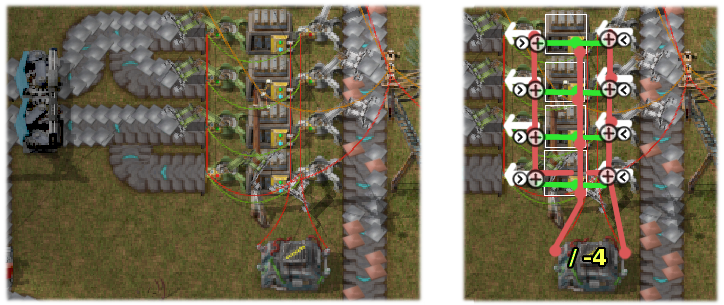
\includegraphics{balancer.png}
\label{And that's how it works.}
\end{figure}

\end{document}
